%%%%%%%%%%%%%%%%%%%%%%%%%%%%%%%%%%%%%%%%%%%%%%%%%%%%%%%%%%%%%%%%%%%%%%%%%%%%%%%%%%
\begin{frame}[fragile]\frametitle{}
\begin{center}
{\Large Introduction}
\end{center}
\end{frame}

%%%%%%%%%%%%%%%%%%%%%%%%%%%%%%%%%%%%%%%%%%%%%%%%%%%%%%%%%%%
\begin{frame}[fragile]\frametitle{Underlying Commonality in Deep Learning}


\begin{itemize}
\item The essence of deep learning is built from two simple algorithmic principles: first, the notion of representation or feature learning, whereby adapted, often hierarchical, features capture the appropriate notion of regularity for each task, and second, learning by local gradient-descent type methods, typically implemented as back-propagation.
\item Core question: ``How do we design deep learning algorithms that are invariant to semantically equivalent transformations while maintaining maximum expressivity?
% \item E.g. for input set ${w,x,y,z}$ and $k=2$ ie 2-tuples, the permutations are $(w,x),(x,w),(w,y), \ldots, (z,y)$.
\item For $k=1$ its a simpler linear model, easy to compute but less expressive.
\item For $k=2$ a bit complex and costly but more expressive.
\item Data may have some inherent 'regularities' (core generation function of sorts). Like creating sample points from a function. If we know this core function, the samples are redundant, meaning more of them does not add value. This is 'inductive bias'.
\end{itemize}
	  
{\tiny (Ref: Geometric Deep Learning Blueprint (Special Edition) - Machine Learning Street talk)}

\end{frame}

%%%%%%%%%%%%%%%%%%%%%%%%%%%%%%%%%%%%%%%%%%%%%%%%%%%%%%%%%%%
\begin{frame}[fragile]\frametitle{From Deep Learning \ldots}


\begin{itemize}
\item Deep Learning model architectures encode inductive biases.
\item Inductive bias is the set of assumptions that the model uses to predict outputs of given inputs that it has not encountered during training, ie unseen data. How can it do that? 
\item [Yogesh] It, while training, some underlying structures, say curve or surface fitting, so that for unseen point, the curve/surface can still predict the output.
\item A classical example of an inductive bias is Occam's razor, assuming that the simplest consistent hypothesis (read, 'fitting', Yogesh) is the best.
\item One of the most powerful inductive biases is to leverage notions of geometry, giving rise to the field of geometric deep learning.
\item So, fundamentally, geometric deep learning involves encoding a geometric understanding of data as an inductive bias in deep learning models to give them a helping hand.
\end{itemize}
	  
{\tiny (Ref: A Brief Introduction to Geometric Deep Learning - Jason McEwen)}

\end{frame}

%%%%%%%%%%%%%%%%%%%%%%%%%%%%%%%%%%%%%%%%%%%%%%%%%%%%%%%%%%%
\begin{frame}[fragile]\frametitle{From Deep Learning \ldots}

Our geometric understanding of the world is typically encoded through three types of geometric priors:

	\begin{itemize}
	\item Symmetry and invariance
	\item Stability
	\item Multi-scale representations
	\end{itemize}


{\tiny (Ref: A Brief Introduction to Geometric Deep Learning - Jason McEwen)}

\end{frame}

%%%%%%%%%%%%%%%%%%%%%%%%%%%%%%%%%%%%%%%%%%%%%%%%%%%%%%%%%%%
\begin{frame}[fragile]\frametitle{From Deep Learning \ldots}

Symmetry, Invariance:

\begin{itemize}
\item If we know the real world exhibits certain symmetries, then it makes sense to encode those symmetries directly into our deep learning model.
\item That way we are able to give the model a helping hand so that is does not have to learn the symmetry but in some sense already knows it.
\item As an example of encoding symmetries and in variances, traditional Convolutional neural networks (CNNs) exhibit what is called translational equivariance.
\item If the camera or cat moves, i.e. is translated in the image, content in the feature space should more similarly, i.e. is also translated. This property is called translational equivariance and in a sense ensures a pattern (cat’s face) need only be learnt once. Rather than having to learn the pattern in all possible locations, by encoding translational equivariance in the model itself we ensure the pattern can then be recognized in all locations.
\end{itemize}

{\tiny (Ref: A Brief Introduction to Geometric Deep Learning - Jason McEwen)}

\end{frame}

%%%%%%%%%%%%%%%%%%%%%%%%%%%%%%%%%%%%%%%%%%%%%%%%%%%%%%%%%%%
\begin{frame}[fragile]\frametitle{From Deep Learning \ldots}

Stability :

\begin{itemize}
\item For a classification problem, for example, small distortions are responsible for variations within a class, whereas larger distortions can map data instances from one class to another. 
\item Small changes to '6' are within class, but a big change to '8' goes to a different class.
\item Stability of the feature mapping is required to ensure such distances are preserved to facilitate effective learning.
\end{itemize}

\begin{center}
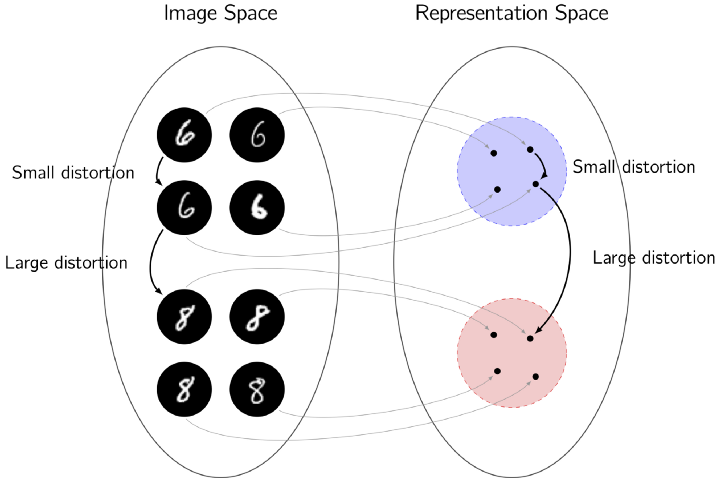
\includegraphics[width=0.5\linewidth,keepaspectratio]{gdl12}
\end{center}

{\tiny (Ref: A Brief Introduction to Geometric Deep Learning - Jason McEwen)}

\end{frame}

%%%%%%%%%%%%%%%%%%%%%%%%%%%%%%%%%%%%%%%%%%%%%%%%%%%%%%%%%%%
\begin{frame}[fragile]\frametitle{From Deep Learning \ldots}

Multi-scale, hierarchical representation of data:

\begin{itemize}
\item Data, many times, are not independent but are correlated in complex ways
\item CE.g. each image pixel is not independent but rather nearby pixels are often related and very similar. [Yogesh] Like 'resolution' or zooming out and zooming in, scaling wise, preserves the structure, say, same as  JPEG-2000 image compression, which compresses but preserves the image content.
\end{itemize}

\begin{center}
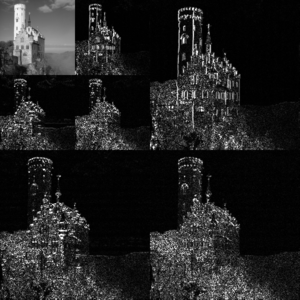
\includegraphics[width=0.3\linewidth,keepaspectratio]{gdl13}
\end{center}

{\tiny (Ref: A Brief Introduction to Geometric Deep Learning - Jason McEwen)}

\end{frame}



%%%%%%%%%%%%%%%%%%%%%%%%%%%%%%%%%%%%%%%%%%%%%%%%%%%%%%%%%%%
\begin{frame}[fragile]\frametitle{It's all about Data}

Training data is of two main domains:
\begin{itemize}
\item Euclidean: Multi-dimensional linear/planar space. Distance between two data-points is a straight line. E.g. tabular data. Current Deep Learning models work very well with this.
\item Non-euclidean: Distance between two data-points is not a straight line. E.g. Social Networks, Meshed 3D surfaces. Recent Geometric Deep Learning are for this type of data.
\end{itemize}
	  
\begin{center}
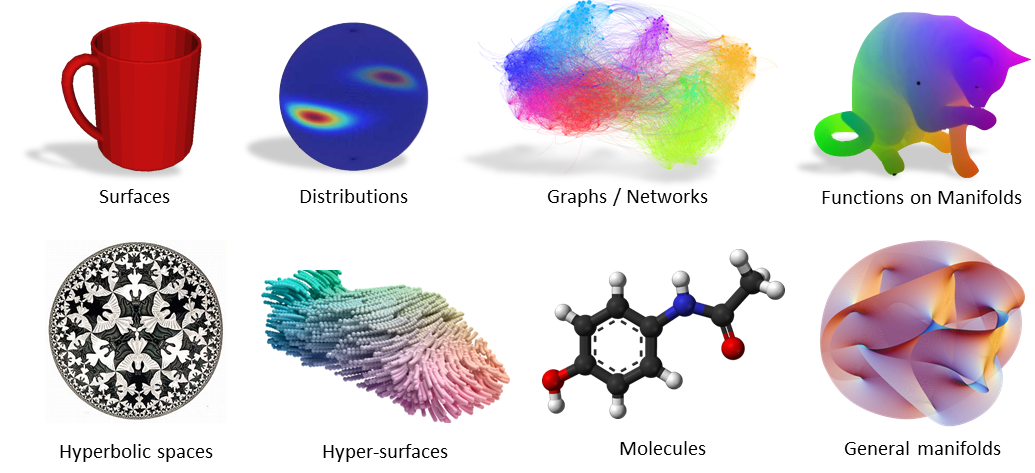
\includegraphics[width=0.8\linewidth,keepaspectratio]{gdl1}
\end{center}

{\tiny (Ref: http://graphics.stanford.edu/courses/cs468-20-fall/)}

\end{frame}


%%%%%%%%%%%%%%%%%%%%%%%%%%%%%%%%%%%%%%%%%%%%%%%%%%%%%%%%%%%
\begin{frame}[fragile]\frametitle{Why Geometric?}

\begin{itemize}
\item Euclidean geometry works on planes. But, say, for curved surfaces, like, earth, the straight line distance between two points in not really the correct (arc) distance.
\item Different types of surfaces, different rules of geometries.
\item Can there be any unification?
\item In 1872, professor Felix Klein started 'Erlangen Program' to unify all these geometries by using the concepts of Invariance and Symmetry.
\end{itemize}
	  
\begin{center}
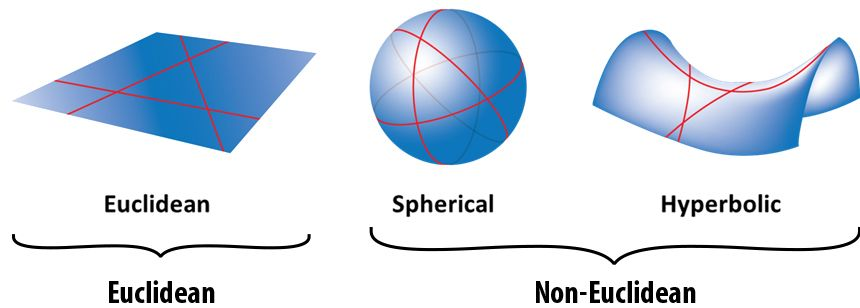
\includegraphics[width=0.8\linewidth,keepaspectratio]{gdl2}
\end{center}

{\tiny (Ref: A gentle introduction to Geometric Deep Learning - Vitale Sparacello)}

\end{frame}

%%%%%%%%%%%%%%%%%%%%%%%%%%%%%%%%%%%%%%%%%%%%%%%%%%%%%%%%%%%
\begin{frame}[fragile]\frametitle{Why Geometric?}

DNNs usually work with fixed-size structured inputs like vectors. Things get complicated with non-Euclidean data
	  
\begin{center}
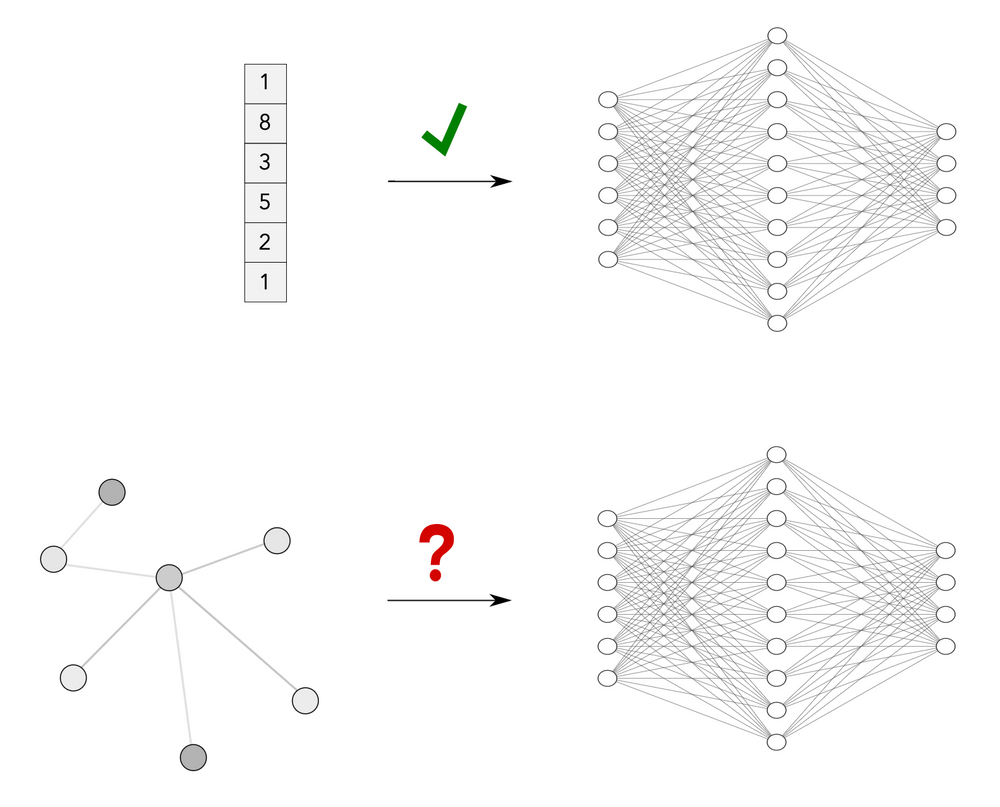
\includegraphics[width=0.6\linewidth,keepaspectratio]{gdl3}
\end{center}

{\tiny (Ref:https://distill.pub/2021/understanding-gnns/)}

\end{frame}

%%%%%%%%%%%%%%%%%%%%%%%%%%%%%%%%%%%%%%%%%%%%%%%%%%%%%%%%%%%
\begin{frame}[fragile]\frametitle{Example: Convolution}

\begin{itemize}
\item Convolutions work well on fixed size images and filters which share weights.
\item How can we formalize and extend this idea for other domains? 
\item Maybe applying geometric principles \ldots
\end{itemize}
	  
\end{frame}

%%%%%%%%%%%%%%%%%%%%%%%%%%%%%%%%%%%%%%%%%%%%%%%%%%%%%%%%%%%
\begin{frame}[fragile]\frametitle{Universal Approximation Theorem}

\begin{itemize}
\item Goal of Machine Learning is to learn a 'function' that approximately fits training data.
\item Universal Approximation Theorem: with just one hidden layer, they can represent combinations of step functions, allowing to approximate any continuous function with arbitrary precision
\end{itemize}
	  
\begin{center}
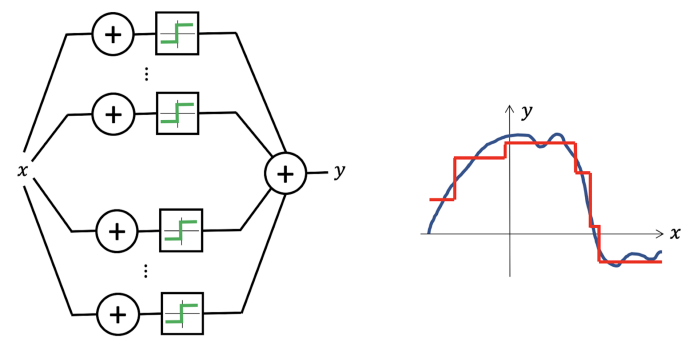
\includegraphics[width=0.8\linewidth,keepaspectratio]{gdl4}
\end{center}

{\tiny (Ref: https://towardsdatascience.com/geometric-foundations-of-deep-learning-94cdd45b451d)}		
\end{frame}

%%%%%%%%%%%%%%%%%%%%%%%%%%%%%%%%%%%%%%%%%%%%%%%%%%%%%%%%%%%
\begin{frame}[fragile]\frametitle{Dimensionality Curse}

\begin{itemize}
\item Things get complicated in high dimensions
\item We need an exponential number of samples to approximate even the most straightforward multidimensional function.
\item Same number of samples but additional dimensionality makes the space so big that the sample dataset becomes very sparse, thus can be statistically insignificant.
\item Example (below) Approximation of a continuous function in multiple dimensions
\end{itemize}
	  
\begin{center}
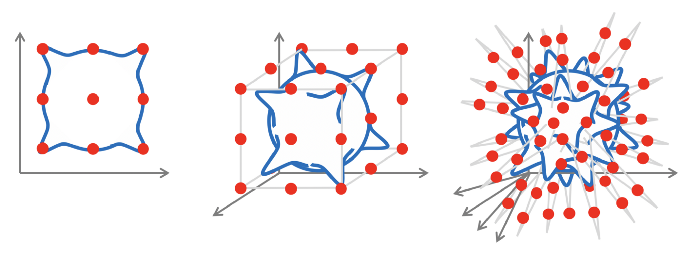
\includegraphics[width=0.8\linewidth,keepaspectratio]{gdl5}
\end{center}

{\tiny (Ref: https://towardsdatascience.com/geometric-foundations-of-deep-learning-94cdd45b451d)}		
\end{frame}

%%%%%%%%%%%%%%%%%%%%%%%%%%%%%%%%%%%%%%%%%%%%%%%%%%%%%%%%%%%
\begin{frame}[fragile]\frametitle{Dimension Reduction}

\begin{itemize}
\item Dimension reduction (by Principal Component Analysis, pCA) can be done, but thats not without losing information.
\item To overcome this problem, we can use the geometric structure of input data. This structure is formally called Geometric prior and it is useful to formalize how we should process the input data.
\end{itemize}
	  
\begin{center}
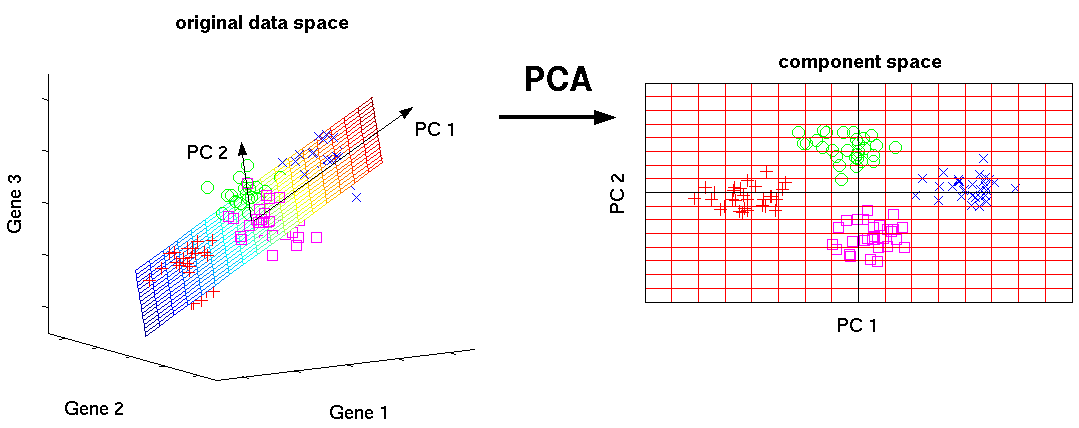
\includegraphics[width=0.8\linewidth,keepaspectratio]{gdl6}
\end{center}

{\tiny (Ref: https://medium.com/@jamesim2077/introduction-to-pca-principal-component-analysis-c26dffe2a857)}		
\end{frame}


%%%%%%%%%%%%%%%%%%%%%%%%%%%%%%%%%%%%%%%%%%%%%%%%%%%%%%%%%%%
\begin{frame}[fragile]\frametitle{Geometric Data}

\begin{itemize}
\item Data based on certain geometrical structure or principle. 
\item For 2D image, its flattened/projected(?) d-dimensional vector of pixels can be its Geometric Prior.
\item Can process images independently of any shift (CNNs)
\item Can process data projected on spheres independently of rotations
\item Can process graph data independently of isomorphism (Graph Neural Networks).
\end{itemize}
	
\end{frame}

%%%%%%%%%%%%%%%%%%%%%%%%%%%%%%%%%%%%%%%%%%%%%%%%%%%%%%%%%%%
\begin{frame}[fragile]\frametitle{What is Graph?}


	  
\begin{center}
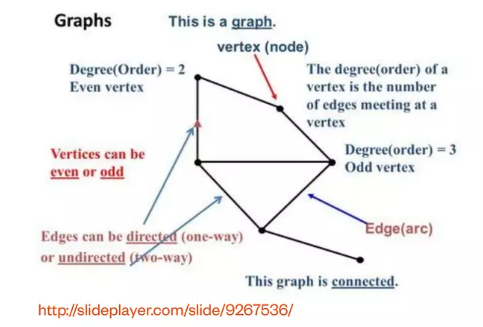
\includegraphics[width=0.8\linewidth,keepaspectratio]{gdl16}
\end{center}

\end{frame}


%%%%%%%%%%%%%%%%%%%%%%%%%%%%%%%%%%%%%%%%%%%%%%%%%%%%%%%%%%%
\begin{frame}[fragile]\frametitle{Graphs, now}

See the progression \ldots

\begin{itemize}
\item In tabular data, rows are independent of each other. E.g. Regression, Classification.
\item In time-series or sequential data, the next point is dependent on previous point(s).
\item In images or spatial data, one point is dependent on the neighbors of fixed size.
\item In social networks, points are connected to each other, do not have order, can have cycle, can have direction, the most generic case, thats Graphs \ldots.
\end{itemize}
	
	{\em Data has shape, and shape has a meaning}
	
\end{frame}


%%%%%%%%%%%%%%%%%%%%%%%%%%%%%%%%%%%%%%%%%%%%%%%%%%%%%%%%%%%
\begin{frame}[fragile]\frametitle{Geometric Deep Learning, the abstraction}

\begin{center}
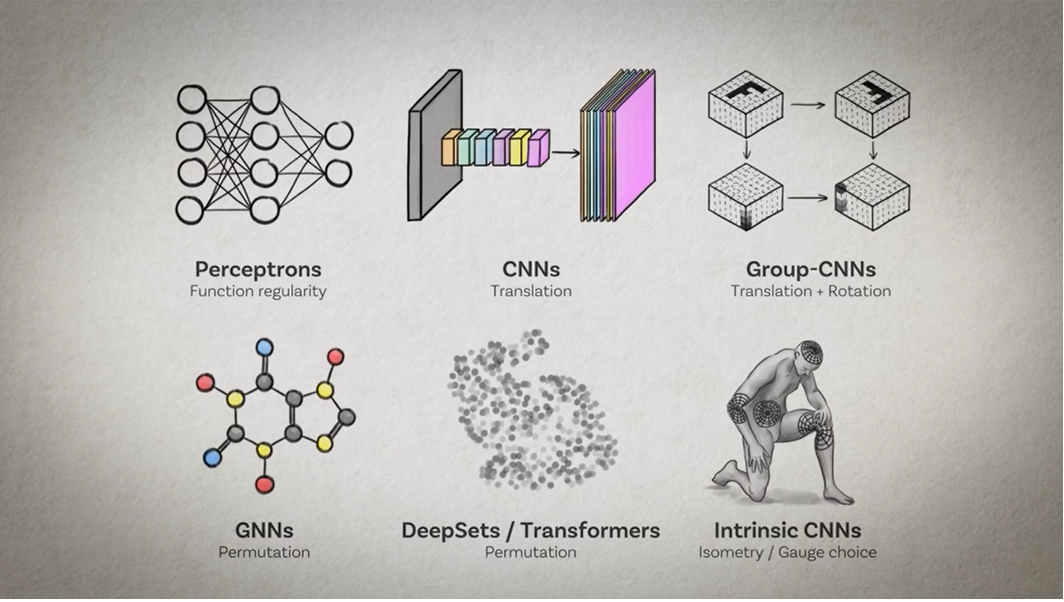
\includegraphics[width=\linewidth,keepaspectratio]{gdl11}
\end{center}

{\tiny (Ref: Geometric Deep Learning Blueprint (Special Edition) - Machine Learning Street talk)}
	
\end{frame}

%%%%%%%%%%%%%%%%%%%%%%%%%%%%%%%%%%%%%%%%%%%%%%%%%%%%%%%%%%%
\begin{frame}[fragile]\frametitle{Categories of Geometric Deep Learning}


\begin{itemize}
\item Grid captures regularly sampled, or gridded, data such as 2D images
\item Group covers homogeneous spaces with global symmetries e.g sphere, not only when data is acquired directly on the sphere (such as over the Earth or by 360° cameras that capture panoramic photos and videos), but also when considering spherical symmetries (such as in molecular chemistry or magnetic resonance imaging). 
\item Graph covers connected data, networks, with nodes and edges.
\item Geodesics and Gauges involve more complex shapes, such as more general manifolds and 3D meshes.
\end{itemize}

\begin{center}
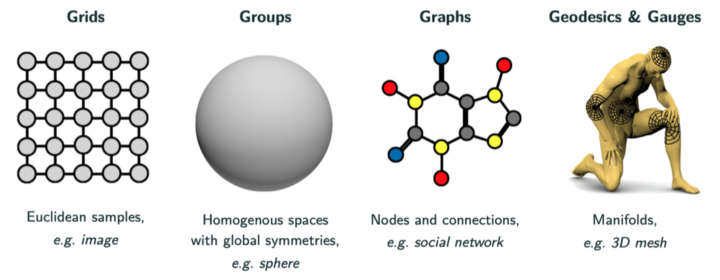
\includegraphics[width=0.8\linewidth,keepaspectratio]{gdl14}
\end{center}

{\tiny (Ref: A Brief Introduction to Geometric Deep Learning - Jason McEwen)}

\end{frame}

%%%%%%%%%%%%%%%%%%%%%%%%%%%%%%%%%%%%%%%%%%%%%%%%%%%%%%%%%%%
\begin{frame}[fragile]\frametitle{Core Principles}
Blueprint of Geometric Deep Learning:
\begin{itemize}
\item Symmetry
\item Scale separation
\item Geometric stability
\end{itemize}

For example, in CNNs
\begin{itemize}
\item Locally equivalent layers, the Convolutional layers
\item Each is followed by coarsening or pooling layers
\item And the last is global invariant pooling layer, say, a classification head.
\end{itemize}
	
\end{frame}

%%%%%%%%%%%%%%%%%%%%%%%%%%%%%%%%%%%%%%%%%%%%%%%%%%%%%%%%%%%
\begin{frame}[fragile]\frametitle{Geometric Deep Learning}

Identifies two main priors our functions must respect to simplify the problem and injecting geometric assumptions to input data:

\begin{itemize}
\item Symmetry: is respected by functions that leave an object invariant, they must be composable, invertible, and they must contain the identity;
\item Scale Separation: the function should be stable under slight deformation of the domain.
\end{itemize}
	
	 If the class of functions we define respect these properties we can tackle any data domain.
	 
\begin{center}
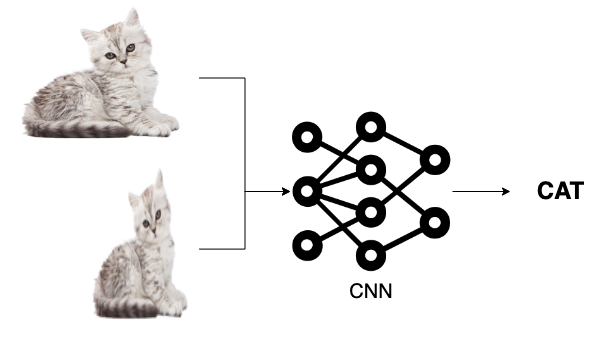
\includegraphics[width=0.6\linewidth,keepaspectratio]{gdl7}
\end{center}

{\tiny (Ref: A gentle introduction to Geometric Deep Learning - Vitale Sparacello)}	
\end{frame}


%%%%%%%%%%%%%%%%%%%%%%%%%%%%%%%%%%%%%%%%%%%%%%%%%%%%%%%%%%%
\begin{frame}[fragile]\frametitle{Symmetry}

\begin{itemize}
\item  A symmetry of an object is simply a transformation of that object which leaves it unchanged.
\item Many symmetries in Deep Learning
\begin{itemize}
\item Weight symmetry: if you exchange weights then still the neural network is graph isomorphic.
\item Label symmetry: the dog is still a dog even if you rotate or translate it.
\end{itemize}
\item If you need all the symmetries (possible variations??) of a class then we would need just one sample to learn. Because all other samples would be semantically equivalent (correlated?).
\end{itemize}


\end{frame}

%%%%%%%%%%%%%%%%%%%%%%%%%%%%%%%%%%%%%%%%%%%%%%%%%%%%%%%%%%%
\begin{frame}[fragile]\frametitle{Symmetry Examples}

\begin{itemize}
\item A symmetry ie a transformation that preserves the structure.
\item E.g. permutations (shuffling) of set members preserves it to be a set.
\item Transformations like rotation and translation preserve relative distance between points.
\item The identity transformation is a symmetry.
\item Composing a symmetric transformation is always a symmetry.
\item Inverse of a symmetry is always a symmetry.
\item This is nothing but a Symmetry Group. 
\item Group, in mathematics, is an abstract way of representing a collection of things, which allow certain set of operations on the members. How members compose with each other.
\end{itemize}
	
\end{frame}


%%%%%%%%%%%%%%%%%%%%%%%%%%%%%%%%%%%%%%%%%%%%%%%%%%%%%%%%%%%
\begin{frame}[fragile]\frametitle{Permutations}

\begin{itemize}
\item  Geometric Deep Learning tries to find functions to be  able to process graph data independently of node organization

\item  All the possible node combinations are defined by a mathematical operation called Permutation. The functions must respect: 
\begin{itemize}
\item Permutation Invariance: applying permutations shouldn’t modify the result. $f(PX,PAP^T )=f(X,A)$
\item Permutation Equivalence: it doesn’t matter if we apply permutations before or after the function. $f(PX, PAP^T)=Pf(X, A)$
\item E.g. in Convolutional Neural Networks (it doesn't matter if pixels are translated) by using Convolutions on pixels neighbors (more formally: using local equivalent processing layers).
\end{itemize}
	\end{itemize}


\end{frame}

%%%%%%%%%%%%%%%%%%%%%%%%%%%%%%%%%%%%%%%%%%%%%%%%%%%%%%%%%%%
\begin{frame}[fragile]\frametitle{Neighborhood}


\begin{itemize}
\item Let’s define the set $N_i$ of the neighbors of node $i$ as $X_{N_i}={x_j: j  N_i}$ ie. $x_1$ has neighbors called $X_{N_1}$
\item E.g. local neighborhood of the node $x_b$ is possible to create hidden representation $h_b$ using the aggregation function $g(x_b, X_{N_b})$.
 
\end{itemize}
	
\begin{center}
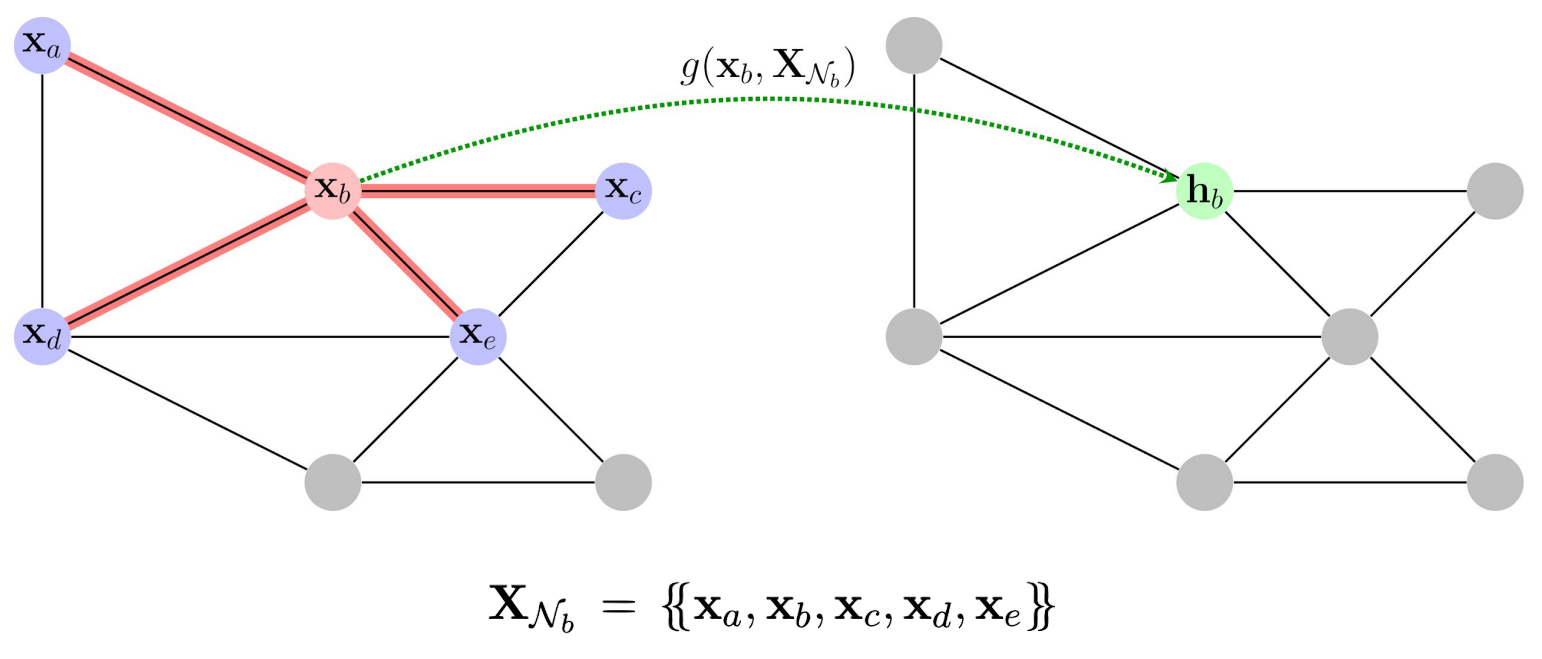
\includegraphics[width=0.6\linewidth,keepaspectratio]{gdl8}
\end{center}

{\tiny (Ref: https://petar-v.com/talks/5G-CS224W.pdf)}	

\end{frame}


%%%%%%%%%%%%%%%%%%%%%%%%%%%%%%%%%%%%%%%%%%%%%%%%%%%%%%%%%%%
\begin{frame}[fragile]\frametitle{Neighborhood Aggregation}

Defining how we compute the latent representations, using the aggregation function $g$ (aka the hidden layers) we can have different flavors of GNNs:

\begin{itemize}
\item Convolutional GNNs: they use the neighbors to compute the hidden representation of the current node. Using this approach is possible to mock CNNs by computing localized convolutions.
\item Attentional GNNs: they use a self attention mechanism similar to Transformer models to learn weights between each couple of connected nodes.
\item Message passing GNNs: they propagate node features by exchanging information between adjacent nodes.
\end{itemize}
	
\begin{center}
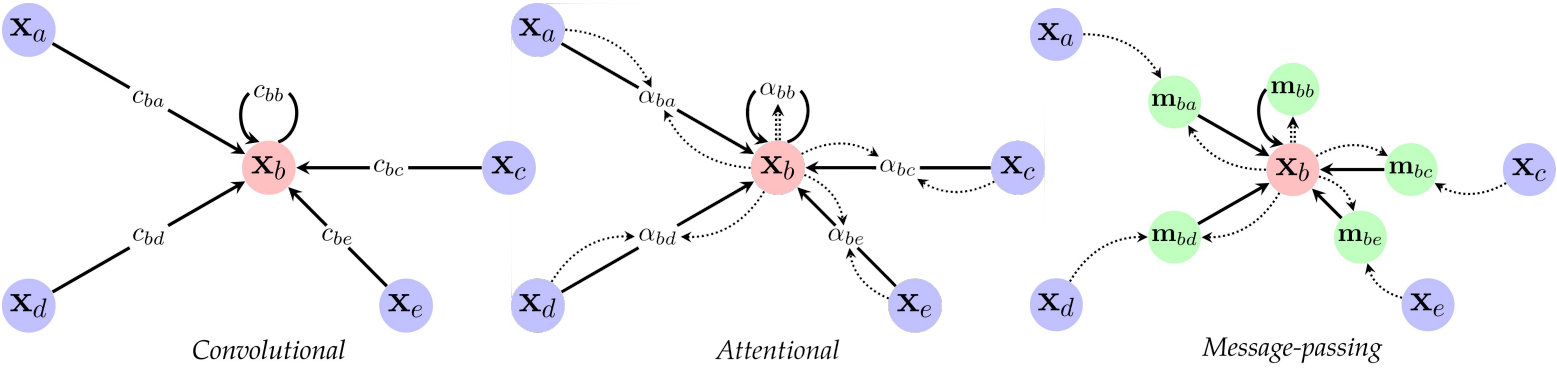
\includegraphics[width=0.6\linewidth,keepaspectratio]{gdl10}
\end{center}

{\tiny (Ref: https://petar-v.com/talks/5G-CS224W.pdf)}	

\end{frame}





%%%%%%%%%%%%%%%%%%%%%%%%%%%%%%%%%%%%%%%%%%%%%%%%%%%%%%%%%%%
\begin{frame}[fragile]\frametitle{Building Blocks/Layers}

Although there are different categories and priors in Geometric Deep Learning, there are some fundamental building blocks/layers.
\begin{itemize}
\item Linear equivariant layers such as convolutions, equivariant to some symmetry transformation. Btw, a convolution on the sphere and graph are difficult
\item Non-linear equivariant layers: To ensure deep learning models have sufficient representational power, they must exhibit non-linearity, while also preserving equivariance.
\item Local averaging such as max pooling layers in CNNs impose local invariance at certain scales, ensuring stability and leading to multi-scale, hierarchical representations by stacking multiple blocks of layers.
\item Global averaging to impose global invariances, such as global pooling layers in CNNs.
\end{itemize}


{\tiny (Ref: A Brief Introduction to Geometric Deep Learning - Jason McEwen)}

\end{frame}

%%%%%%%%%%%%%%%%%%%%%%%%%%%%%%%%%%%%%%%%%%%%%%%%%%%%%%%%%%%
\begin{frame}[fragile]\frametitle{Application}


\begin{itemize}
\item Deep Graph Neural Networks are built by stacking multiple of these layers!
\item Using this blueprint is possible to train GNNs able to solve the following tasks:
\end{itemize}
	
\begin{center}
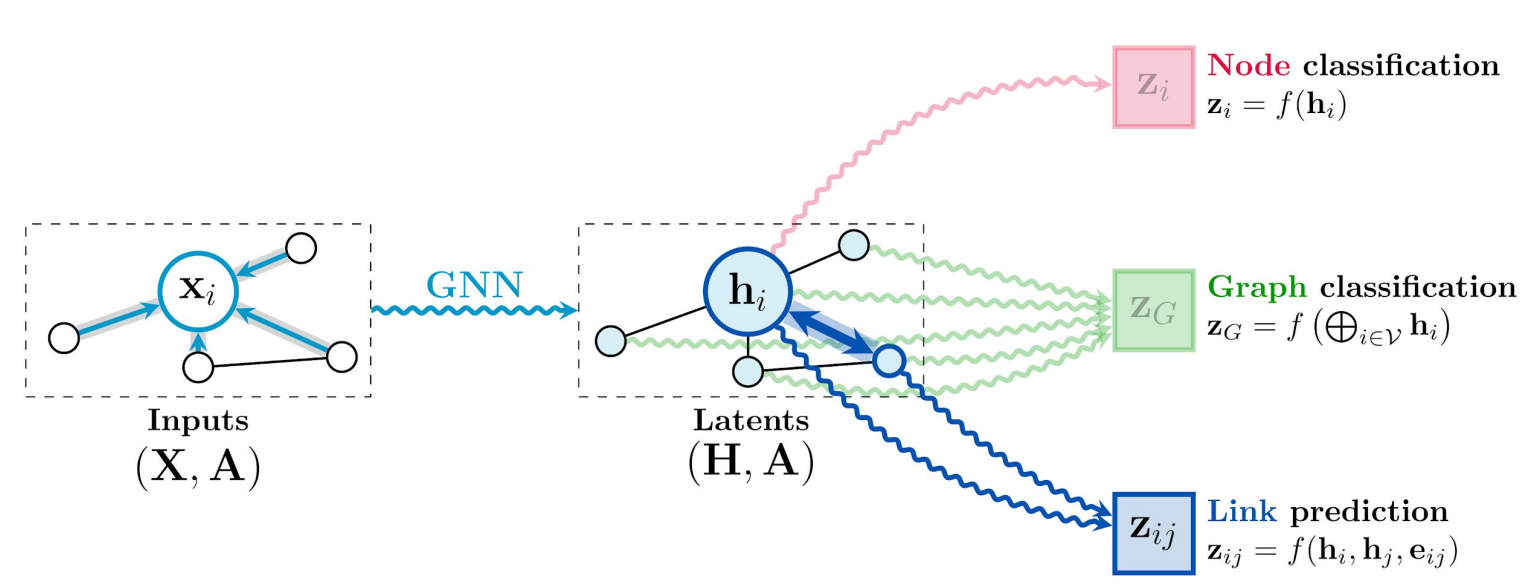
\includegraphics[width=0.6\linewidth,keepaspectratio]{gdl9}
\end{center}

{\tiny (Ref: https://petar-v.com/talks/5G-CS224W.pdf)}	

\end{frame}


%%%%%%%%%%%%%%%%%%%%%%%%%%%%%%%%%%%%%%%%%%%%%%%%%%%%%%%%%%%
\begin{frame}[fragile]\frametitle{Example: CNN}

Traditional CNN for 2D planar images shows all the building blocks/layers

\begin{center}
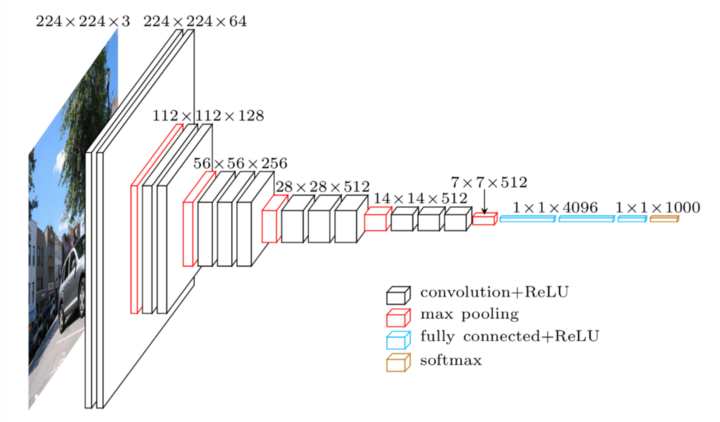
\includegraphics[width=\linewidth,keepaspectratio]{gdl15}
\end{center}


{\tiny (Ref: A Brief Introduction to Geometric Deep Learning - Jason McEwen)}

\end{frame}




%%%%%%%%%%%%%%%%%%%%%%%%%%%%%%%%%%%%%%%%%%%%%%%%%%%%%%%%%%%
\begin{frame}[fragile]\frametitle{Conclusion}

\begin{itemize}
\item Geometric deep learning is a topical and rapidly evolving field
\item  While learning generic functions in high dimensions is a cursed estimation problem, most tasks of interest are not generic, and come with essential pre-defined regularities arising from the underlying low-dimensionality and structure of the physical world. 
\item This topic is  exposing these regularities through unified geometric principles that can be applied throughout a wide spectrum of applications.
\item Such a 'geometric unification' endeavor, in the spirit of Felix Klein's Erlangen Program, serves a dual purpose: 
\begin{itemize}
\item  provides a common mathematical framework to study the most successful neural network architectures, such as CNN's, RNNs, GNNs, and Transformers
\item gives a constructive procedure to incorporate prior physical knowledge into neural architectures and provide a principled way to build future architectures yet to be invented
	\end{itemize}
	\end{itemize}

{\tiny (Ref: Geometric Deep Learning, LinkedIn post by Ashish Patel)}

\end{frame}

%%%%%%%%%%%%%%%%%%%%%%%%%%%%%%%%%%%%%%%%%%%%%%%%%%%%%%%%%%%
\begin{frame}[fragile]\frametitle{Why Me?}

\begin{itemize}
\item Confluence of Graphs and Geometry into Deep Learning, my IKIGAI and Specific Knowledge.
\item Demand, both academically \& professionally, as ML will be better on small but connected data.
\item PyTorch Geometric is a beautiful, production-ready, research-heavy and good expertize-skill to have.
\end{itemize}
	  
\end{frame}


%%%%%%%%%%%%%%%%%%%%%%%%%%%%%%%%%%%%%%%%%%%%%%%%%%%%%%%%%%%
\begin{frame}[fragile]\frametitle{References}

\begin{itemize}
\item A gentle introduction to Geometric Deep Learning - Vitale Sparacello
\item ``Geometric Deep Learning Blueprint (Special Edition)'' - Machine Learning Street Talk
\item Geometric Deep Learning: Grids, Groups, Graphs, Geodesics, and Gauges
https://arxiv.org/abs/2104.13478
\item A Brief Introduction to Geometric Deep Learning - Jason McEwen
\end{itemize}
	  
\end{frame}
